\documentclass{article}

\usepackage[utf8]{inputenc}
\usepackage[english]{babel}
\usepackage[english]{isodate}
\usepackage[parfill]{parskip}
\usepackage{graphicx}
\usepackage{amsmath}
\usepackage{listings}
\usepackage[hidelinks]{hyperref}
\usepackage{fixltx2e}
\usepackage{listings}

\setcounter{tocdepth}{4}
\setcounter{secnumdepth}{4}

\setlength\parindent{24pt}

\title{Camera Calibration}
\author{Nick Weidner}

\newcommand*{\titleGM}{\begingroup % Create the command for including the title page in the document
	\hbox{ % Horizontal box
		\hspace*{0.2\textwidth} % Whitespace to the left of the title page
		\rule{1pt}{\textheight} % Vertical line
		\hspace*{0.05\textwidth} % Whitespace between the vertical line and title page text
		\parbox[b]{0.75\textwidth}{ % Paragraph box which restricts text to less than the width of the page
			
			{\noindent\Huge\bfseries Camera Calibration \\[0.5\baselineskip] A User's Guide}\\[2\baselineskip] % Title
			{\large \textit{}}\\[4\baselineskip] % Tagline or further description
			{\Large \textsc{Nick Weidner}} % Author name
			
			\vspace{0.5\textheight} % Whitespace between the title block and the publisher
			{\noindent  \plogo}\\[\baselineskip] % Publisher and logo
}}
\endgroup}

\begin{document}
\pagestyle{empty}
\titleGM
\iffalse
\begin{titlepage}
	\vspace*{\stretch{1.0}}
	\begin{center}
		\Large\textbf{Camera Calibration, User's Guide}\\
		\large\textit{Nick Weidner}
	\end{center}
	\vspace*{\stretch{2.0}}
\end{titlepage}
\fi
	
\pagenumbering{Roman}
\tableofcontents
\newpage
\listoffigures
\newpage
\pagenumbering{arabic}

\section{Preface}

Camera Calibration is the backbone, and often first step in any project involving imaging from a camera. Images that are not corrected to account for camera parameters that cause distortion and misalignment are incorrect 2D mappings af the physical world. This means any spatial calculations made with these raw images will inaccurate. When correcting these images, it is practically impossible to accurately calculate a correction with zero error in the pixel values. Any error present can thus compound with all the later error accumulated from future calculations. This is why camera calibration is such a vital first step when working with images. While it may be considered by many to be a long and solved problem, no two data sets are one hundred percent alike. It is important to calibrate carefully, minimize error, and not take the process for granted unless ensue headaches down the road. 

This user's guide is structured to give anyone an overview of the tools out there, and approaches to use to get the best results when calibrating a camera. The two primary packages recommended here are OpenCV and the Matlab Computer Vision System Toolbox. There are a few other Matlab packages and other standard coding library packages out there that can do camera calibration, but they all work similarly on a fundamental level and this guide will address why these are highlighted and when to use which one. It is highly recommended to look over the underlying theory of camera calibration addressed in this guide as well. Many obstacles such as input and output problems can be easily resolved if one understand what goes on behind the scenes and avoids simply calling library functions and expecting an output. 

\section{Underlying Theory}

There are numerous resources on camera calibration in books, in papers, and across the web. A general overview is given here.

\subsection{Pinhole Camera}

We calibrate a camera to identify data on it's most important components. Important for image work at least. These components are...

\begin{itemize}
	\item Focal Length
	\begin{itemize}
		\item The distance from the center of a lens to the focus in the camera
	\end{itemize}
	\item Principal Point
	\begin{itemize}
		\item The location on the image from which the perspective is centered, usually the center of the image.
	\end{itemize}
	\item Distortion 
	\begin{itemize}
		\item How the image changes when it is projected through a lens
	\end{itemize}
	\item Base Line (in stereo systems)
	\begin{itemize}
		\item The distance between the focus of the left and right camera
	\end{itemize}
\end{itemize}
	
If we simplify our system to a pinhole camera model with no lens, then the 3D world maps to a 2D one like this. 

\begin{figure}[h]
	\centering
	\fbox{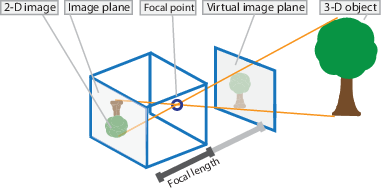
\includegraphics{./figures/camera_calibration_focal_point.png}}
	\caption{Pinhole camera model}
	\label{fig:pinhole}
\end{figure}

The model itself is mathematically represented as...

\[
sm' = A[R|t]M'
\]

or

\[ s 
\left[\begin{array}{c} u \\ v \\ 1 \end{array} \right]
=
\begin{bmatrix}
f_x & 0 & c_x \\ 0 & f_y & c_y \\ 0 & 0 & 1
\end{bmatrix}
\begin{bmatrix}
r_{11} & r_{12} & r_{13} & t_1 \\ r_{21} & r_{22} & r_{23} & t_2 \\ r_{31} & r_{32} & r_{33} & t_3
\end{bmatrix}
\left[\begin{array}{c} X \\ Y \\ Z \\ 1 \end{array} \right]
 \]
 
where:

\begin{itemize}
	\item (X,Y,Z) are coordinates of a 3D point in the world
	\item (u,v) are the coordinates of the same point projected as a pixel on the image
	\item (cx,cy) are the principal point coordinates
	\item fx, fy are the focal lengths in pixel units
\end{itemize}

The A matrix is often regarded as the camera matrix or a matrix of intrinsic parameters. These are the parameters within the camera itself. The \lstinline![R|t]! matrix is a matrix of extrinsic parameters and is used to describe the camera motion around a static scene in regards to rotation and translation. \lstinline![R|t]! translates coordinates of a point in (X,Y,Z) to a coordinate system that is fixed with respect to the camera. 

Using this simple model, a 3D coordinateat (X,Y,Z) can be represented as pixel coordinates u,v as...

\begin{align*}
u&=f_x \times \frac{X}{Z} + c_x & v&=f_y \times \frac{Y}{Z} + c_y
\end{align*}

\subsection{Distortion}

No modern day camera is as simplistic as a pinhole model, and the lens used introduces a wide variety of distortions. The most common forms of distortion arise from radial and tangential distortion. Radial distortion the distortion of light through the lens that causes the image to change it's shape. Tangential distortion is the distortion that arises when a cameras parts are not manufactured directly in line with each other, and the lens and sensor are not completely parallel. Tangential distortion is often minimal, but still worth taking into account. Radial distortion is often much more dramatic, and almost all cameras use a different enough lens that no two cameras have an identical mapping. 

Radial primarily shows up in these forms...

\begin{figure}[h]
	\centering
	\fbox{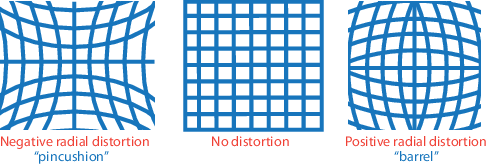
\includegraphics{./figures/calibration_radial_distortion.png}}
	\caption{Radial Distortion}
	\label{fig:radial}
\end{figure}

Barrel and pincushion distortion are mathematically quadratic and can be described by a quadratic polynomial. Depending on the exact shape of a physical lens,  quadratic system may not fit the shape exactly and a higher degree even polynomial fits better. Note an odd degree polynomial would not fit the shape of a lense.  Most practical lenses don't follow a degree higher than 6 because the distortion at a higher degree becomes so minimal. 

These distortions alter our pinhole model to...

\begin{align*}
x'&= X/Z & y'&= Y/Z & r^2 &= x'^2 + y'^2
\end{align*}

\[
x'' = x' \frac{1+k_1r^2+k_2r^4+k_3r^6}{1+k_4r^2+k_5r^4+k_6r^6} + 2p_1x'y' + p_2(r^2 + 2x'^2)
\]

\[
y'' = y' \frac{1+k_1r^2+k_2r^4+k_3r^6}{1+k_4r^2+k_5r^4+k_6r^6} + p_1(r^2+2y'^2) + 2p_2x'y'
\]

\begin{align*}
u &= f_x \times x'' + c_x & v&=f_y \times y'' + c_y
\end{align*}

Where k\textsubscript{1},k\textsubscript{2},... are the radial distortion values and p\textsubscript{1} and p\textsubscript{2} are the tangential distortion values. The equation shown above is specifically the underlying model for OpenCV camera calibration depending on whether the user wants 2, 3, or all 6 coefficients calculated. It is worth noting that the Matlab computer vision system toolbox uses the same model, but only uses 2 to 3 radial coefficients depending on the severity of the distortion. Both are based on the widely famous Brown-Conrady model for which takes in n radial distortion coefficients. 

An alternative distortion model has also been introduced in OpenCV called the fisheye camera model. This model alters the pinhole model to...

\begin{align*}
x'&= X/Z & y'&= Y/Z & r^2 &= x'^2 + y'^2 & \theta &= atan(r)
\end{align*}

\[
\theta_d = \theta(1+k_1\theta^2+k_2\theta^4+k_3\theta^6+k_4\theta^8)
\]

\begin{align*}
x'' &= \frac{\theta_d}{r} \times X & y'' &= \frac{\theta_d}{r} \times Y
\end{align*}

\begin{align*}
u &= f_x \times x'' + c_x & v&=f_y \times y'' + c_y
\end{align*}

This model lacks descriptive documentation of its behind the scenes in OpenCV, but it is based on a more generic camera model and calibration method for wide angle lenses. This has also been  implemented in another Matlab calibration package called the Camera Calibration Toolbox for Matlab.

\subsection{Calibration}

These models are great for transforming world points when we know all of the values, but the whole point of calibrating a camera is that we don't know what any of these values are. This is where the packages come into play. The functions in these packages are designed to take in points from the world and solve a curve fitting problem in order to identify the parameters that most accurately project a point. If not careful, curve fitting problems can inaccurately return solve for a local minimum. This means that parameters can be found that fit our data really well, but work horribly on additional data sets. This makes choosing the data sets very important and will be addressed more in depth later on. In the end, the values we return as our best fit for our data, are going to give off pixel error. This error states how many pixels off from where it should be a pixel is when run through our model. 

\subsection{Stereo}

When introducing another camera into the mix there are a few additional things to consider and calculate. The individual calibration still needs to be done and this is still done independently, nothing in this process is effected by the other camera. Once calibrated, though, the cameras need to be rectified, which means they need to be aligned either horizontally or vertically depending on their orientation. This creates a new camera matrix following the form...
	
\begin{align*}
C1 &=
\begin{bmatrix}
f_x & 0 & c_{x1} & 0\\ 0 & f_y & c_y & 0\\ 0 & 0 & 1 & 0
\end{bmatrix} &
C2 &=
\begin{bmatrix}
f_x & 0 & c_{x2} & T_x \times f\\ 0 & f_y & c_y & 0 \\ 0 & 0 & 1 & 0
\end{bmatrix}
\end{align*}

This is for the case of horizontal stereo and T\textsubscript{x} represents a horizontal shift in the cameras.This is important for calculating a disparity map which identifies the spacial differences of each pixel between the left and right image. 

\section{Getting Started}

Before starting camera calibration, a few things need to be set up and the proper tool for the job needs to be decided on. 

\subsection{Picking the Proper Tool}

In most cases, the basic OpenCV camera calibration functions will easily get the job done. Most cameras calibrate through a very straightforward pipeline and return good results. This is a good place to start if you are unsure. Calibration gets tricky when there is a significant amount of distortion in the camera lens. A fisheye or wide angle lens can sometimes return large error values on the standard OpenCV calibration functions. The OpenCV fisheye calibration functions work nicely here.

 Sometimes the distortion is so dramatic, though, OpenCV struggles to minimize the error. At least not without an exceedingly long and tedious testing process from the user. This is where Matlab shines. The Matlab computer vision system toolbox calibration tool has a built in error plot that helps you identify bad input images. There is no tool for OpenCV directly, so all images must be hand picked. This is usually fairly straight forward, but not on extremely distorted images. 
 
 The GoPro superview camera mode is an example of where Matlab is able to minimze the error, but not OpenCV. If using a GoPro camera make sure to check what mode the recording is done in. Superview is the default on some models, yet it serves practically no purpose when calibration needs to be done because the edges are eventually cropped down to the non superview size anyway and error is much better without it. Here is a short pro and con list of OpenCV vs Matlab.  

\begin{align*}
\begin{tabular}{r|p{0.4\textwidth}}
	OpenCV \\
	Pros & \begin{itemize}
		\item Open source
		\item Very configurable to needs of project
		\item Output is readily available and coincides with other Opencv functions 
		\item Both the standard and fisheye models operate in similar manners 
	\end{itemize} \\
	Cons & \begin{itemize}
		\item Input of images can be tedious
		\item Debugging can be more complicated 
		\item Configurability can make simple things overly confusing
		\item Fails on extremely distorted image sets like the GoPro superview
	\end{itemize}
\end{tabular}
\begin{tabular}{r|p{0.4\textwidth}}
	Matlab \\
	Pros & \begin{itemize}
		\item Easy to set up and use
		\item Easy to combine with other matlab functions 
		\item Error plotting tool makes image selection less tedious
		\item Has success on more distorted image sets like the GoPro superview
	\end{itemize} \\
	Cons & \begin{itemize}
		\item Requires a Matlab license and a package license for the tool
		\item Output data is tedious to use outside of Matlab
		\item Undistortion must be done in Matlab as well
	\end{itemize}
\end{tabular}
\end{align*}

Keep in mind what you intend to do with your data after the camera has been calibrated. If Matlab has all the functionality for what you are trying to do, it is probably easier to do everything in it. If you intend to use OpenCV later down the road, getting the proper results can be tedious from Matlab. For example, undistorted images can be produced with the undistorted parameters at any time once calculated. Matlab undistorts the images differently so any new image set using Matlab calibration parameters has to be run through matlab. There may be a way to do this properly in OpenCV, but none that I could find. 

\subsection{Setting Up}

To start using the Matlab tool, all that is required is Matlab version R2013b or later, and the Computer Vision System Toolbox. The full documentation for the tool can be found at \url{http://www.mathworks.com/help/vision/index.html}

For OpenCV, OpenCV 2.4 or 3.1 should be downloaded from \url{http://opencv.org/downloads.html}. This guide was written with OpenCV 3.1 in mind. I recommend having multiple installs on your machine in case anything comes up that is version specific. You should also download cmake from \url{https://cmake.org/} and create a CMakeList.txt like the following for your project.


\begin{lstlisting}[language=python, frame=single]
cmake_minimum_required(VERSION 3.1)
project( DisplayImage )
find_package( OpenCV REQUIRED )
add_executable( calibration calibration.cpp )
target_link_libraries( calibration ${OpenCV_LIBS} )
\end{lstlisting}

Some may prefer using python with OpenCV which has all of the camera calibration functions available as well. Python is much easier to get up and running quickly and the logical flow of the C++ code is the same. Keep in mind that when using the fisheye model, some of the python functions I found broken. 

The input for camera calibration can be either video or a series of images. Calibration works on a frame by frame basis so they is not much difference. There is a slight distinction, though. When reading video you either need to process every frame or a subset of frames across a common interval. This does not guarantee the optimal selection of input images, so it is recommended to separate videos out frame by frame and compile a set of input images. Matlab requires you to do this as there is no read video option in the toolbox. 

\section{Calibration Input}

Most of the making of breaking of good camera calibration comes from the input parameters. This section will look at how to choose good data, and common errors to avoid when doing so. 

\subsection{Brief Overview}

As mentioned before, calibration algorithms work by curve fitting and equation based on a set of input data. This input data is collected using a camera calibration board. 

\begin{figure}[h]
	\centering
	\fbox{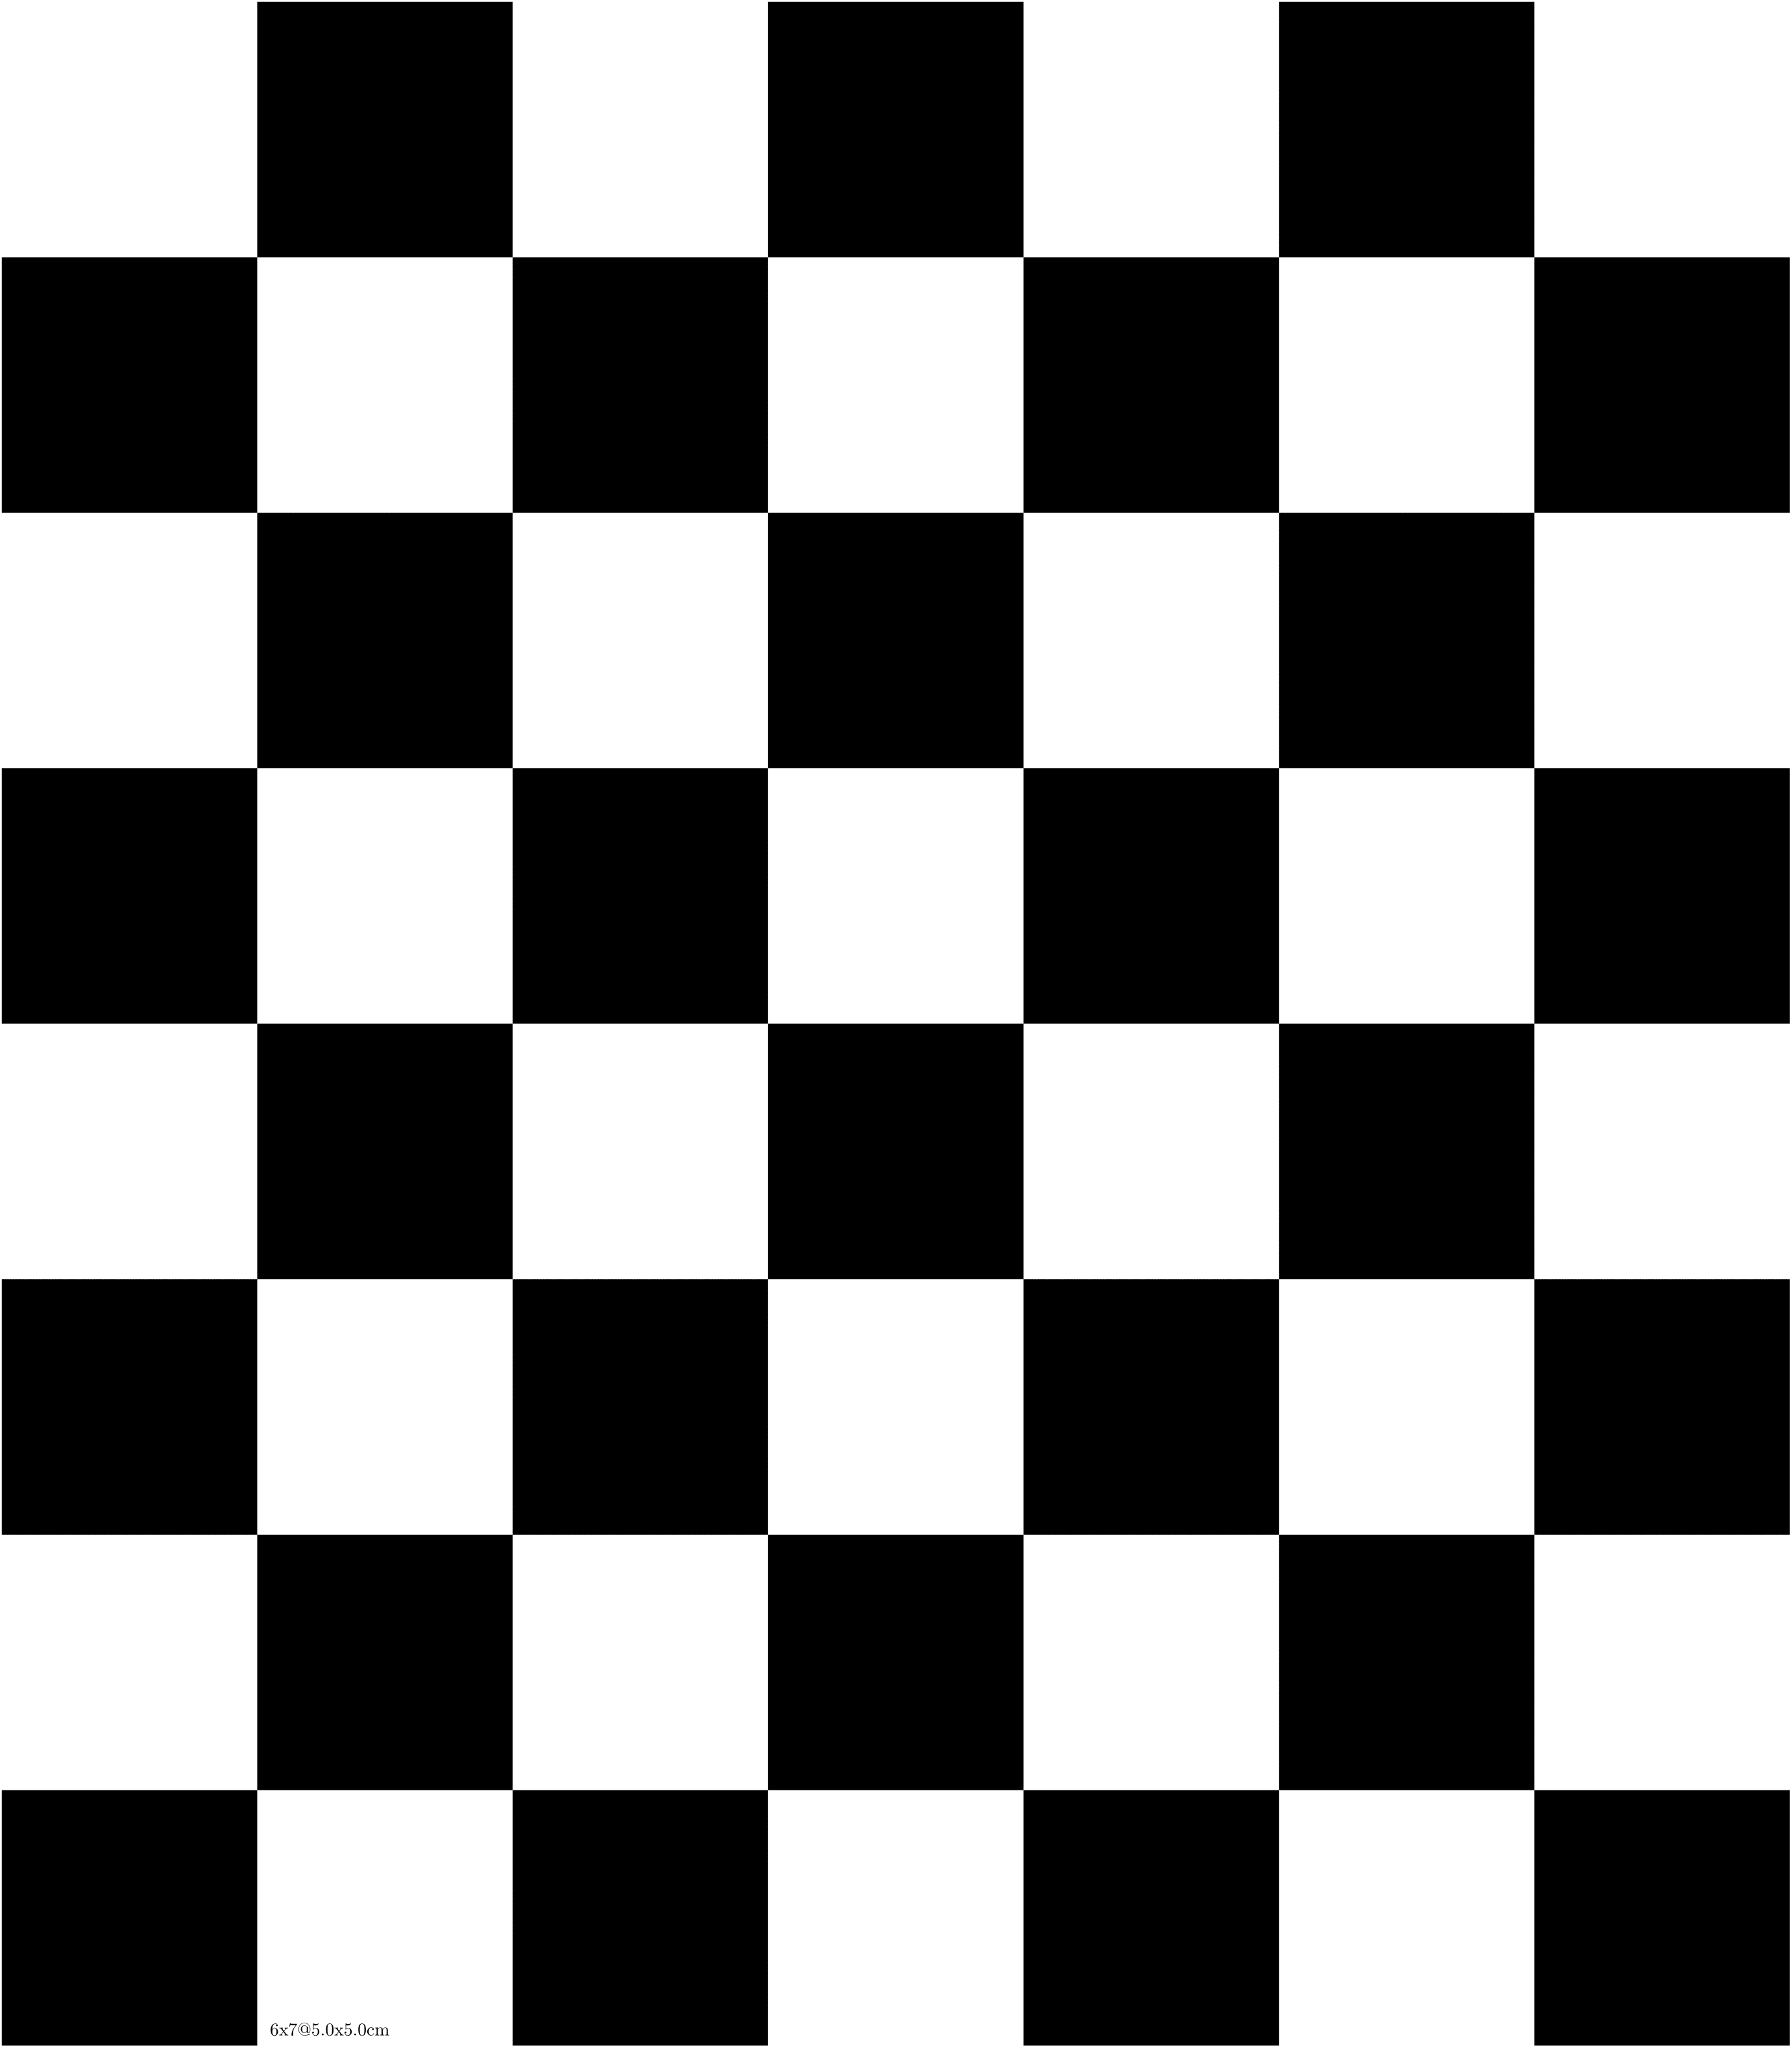
\includegraphics[width=0.45\textwidth]{./figures/checkerboard_7x6_50x50cm-1.png}}
	\caption{7x6 Calibration Board}
	\label{fig:board}
\end{figure}

Using corner detection functions built into OpenCV and Matlab, we can identify the pixel coordinates of board corners on an image taken with a printed one. Taking images when the board is positioned at different distances, positions, and orientations, these corner points provide input for which coefficients can be fit to. 

\subsection{Picking Images}

To avoid the problem of local minimum that was discussed earlier, a wide range of board orientations should be used as input images. Calibration will work on a single image, but for any other images the undistorted will be horribly wrong. A good choice of input images are ones that cover the entirety of the image plane at a range of distances and orientations. This is an example of a low error image set I used to calibrate our underwater stereo rig cameras. 

\begin{figure}[h]
	\centering
	\fbox{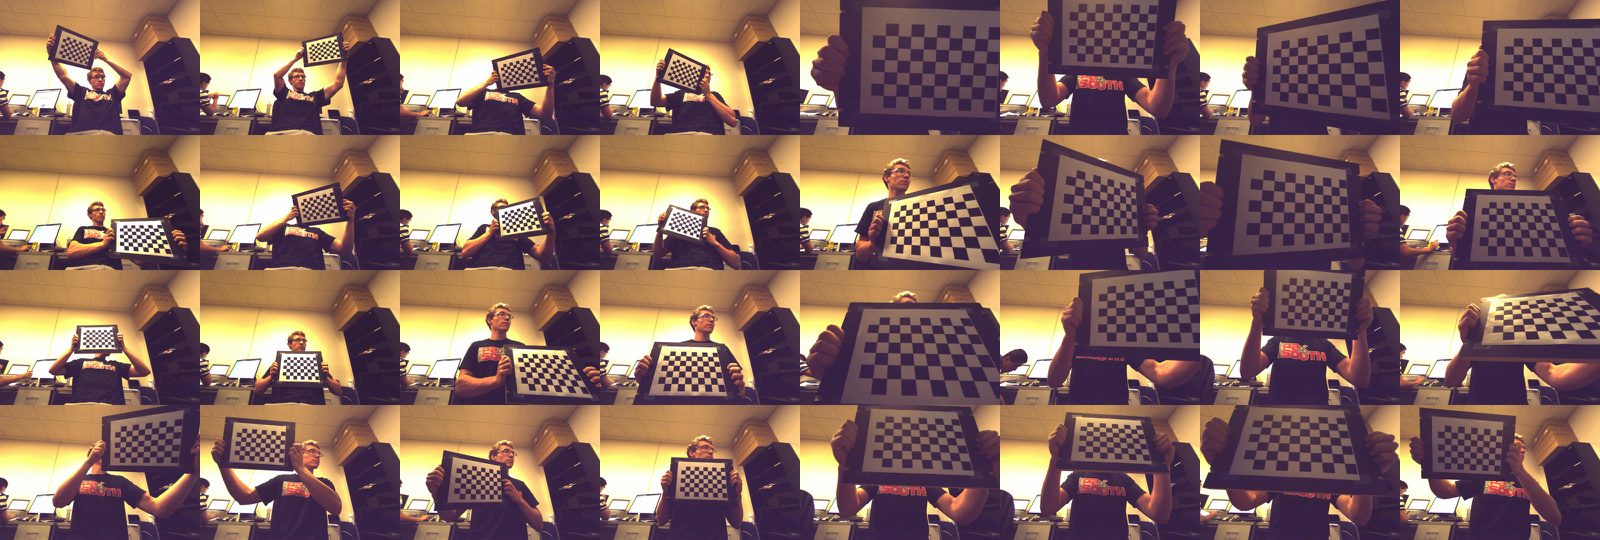
\includegraphics[width=1\textwidth]{./figures/combine_images_final.jpg}}
	\caption{Mosaic of Good input images used}
	\label{fig:cornerselect}
\end{figure}

The most valuable ranges are the very close up and medium distance ranges since they cover the most image space. Ideally, try and get images of the board flat in the center, edges, and corners, and angled a few ways in the center, edges and corners both both distance ranges. You can also get a few at a farther distance. Ideally check the error you are getting with your image set and adjust accordingly. Preferred pixel error is less than 0.5. Anything larger than 1 should be examined for missing image coverage positions and anything larger than 5 probably needs a complete reexamining of the set.

There are a few problems that some times come up and can be easily avoided. Later on in calibration, points are oriented either horizontally or vertically and often for ease of use the entire set is oriented the same way. To avoid breaking calibration, keep the board either horizontal or vertical the entire time. Still angle it slightly to get data from skew, but don't angle it dramatically enough to throw off the orientation. 

To avoid any possible error accumulation, try and keep keep the board as flat as possible. It printed and attached to a surface, try and remove all wrinkles and bubbles underneath. Also move the board at a slow enough speed to avoid motion blur. Blurriness will hurt the accuracy of your corner collection and thus cause error in the calibration. 

Sometimes corners can be found to have one orientation on one image, and an upside down orientation on another. this breaks calibration so it is advised to print an odd by even numbered calibration board which looks difference when flipped 180 degrees around.

A reminder on stereo systems that the corners should be found in both the left and right images. For stereo calibration, both input sets need to be the same to line up or rectification could break. Going to the edge of one camera in a stereo system often cuts off corners from the other, so be wary. If possible, it is much easier to collect a good data set if you can view the video feed as it records. This way you can avoid moving outside the frame of either camera. 

\subsection{Corner Detection}

Corner detection in Matlab is simple. Given a directory with all the input images, specify the directory path and the physical distance between corner points in the units of choosing to the single or stereo calibration application and run. This will output all the found corners of which you can select to delete ones you deem inappropriately selected before calibrating. 

In OpenCV there is a little more involved. Assume we are working with a stereo system, but in a single camera system the process is the same with half the calls. All of this is also in the documentation found \url{http://docs.opencv.org/3.0-beta/modules/calib3d/doc/camera_calibration_and_3d_reconstruction.html}

\begin{lstlisting}[language=C++, frame=single, breaklines]
Size boardSize = Size(7,6);

bool lFoundCorner = false;
bool rFoundCorner = false;

lFoundCorner = findChessboardCorners(leftImage, boardSize, lCorners, CALIB_CB_ADAPTIVE_THRESH|CALIB_CB_NORMALIZE_IMAGE);
rFoundCorner = findChessboardCorners(rightImage, boardSize, rCorners, CALIB_CB_ADAPTIVE_THRESH|CALIB_CB_NORMALIZE_IMAGE);

if ( lFoundCorner && rFoundCorner ) {
	cornerSubPix(leftImage, lCorners, Size(11,11), Size(-1,-1),TermCriteria(TermCriteria::MAX_ITER|TermCriteria::EPS,30, 0.01));
	cornerSubPix(rightImage, rCorners, Size(11,11), Size(-1,-1),TermCriteria(TermCriteria::MAX_ITER|TermCriteria::EPS,30, 0.01));
	
	leftImagePoints.push_back(lCorners);
	rightImagePoints.push_back(rCorners);
	
	objectPoints.push_back(objectPoint);
}
\end{lstlisting}

This is run for each image read in and saved to leftImage and rightImage. The findChessboardCorners function identifies a board of size boardSize, does some adaptive thresholding and normalizing on the image to make it easier to identify corners, and then stores a vector of 2D points in lCorners and rCorners. This function returns a boolean so we know if it successfully found every point. To improve the accuracy of our calibration we calculate everything to subpixel accuracy using cornerSubPix. We add our vector of corner points to a vector of all sets of corner points across all the images to later calibrate across. Finally we add an objectPoint to a vector growing at the same rate as our corner points. These are the calibration pattern points in the calibration pattern coordinate space. We fill it earlier like this. 

\begin{lstlisting}[language=C++, frame=single, breaklines]
float squareWidth = 2.5;
float squareHeight = 2.5;

for (int i =0; i<6; i++) {
	for (int j = 0; j<7; j++) {
		objectPoint.push_back(Point3d(squareWidth*float(j),squareHeight*float(i),0));
	}
}
\end{lstlisting}

The width and height correlate to the actual board size in the unit of choice. In this case 2.5mm. This gives all the calculations physical grounding and creates a mapping between pixel distance and physical distance. It is important here that the height and width line up properly both in the size of each for loop and the value being multiplied. It was mentioned that the board should stay either horizontal or vertical the entire time. These points must line up with that direction or calibration will fail.

\section{Calibration}

With corners collected, there is now a data set to run through calibration. Assuming stereo again, we will now look at running the calibration. Running the calibration is often a straightforward practice, the most common problems come from bad data sets, or setting up something properly. 

\subsection{Matlab calibration}

Much like the other Matlab steps, the process is straightforward. With the bad calibration images removed by the user, select the parameters used for calibration. Radial distortion can be calculated using 2 or 3 coefficients, and it is recommended 3 be used when the distortion is more extreme. Also check whether or not the skew or tangential distortion should be calculated as well. Then select calibrate. 

\begin{figure}[h]
	\centering
	\fbox{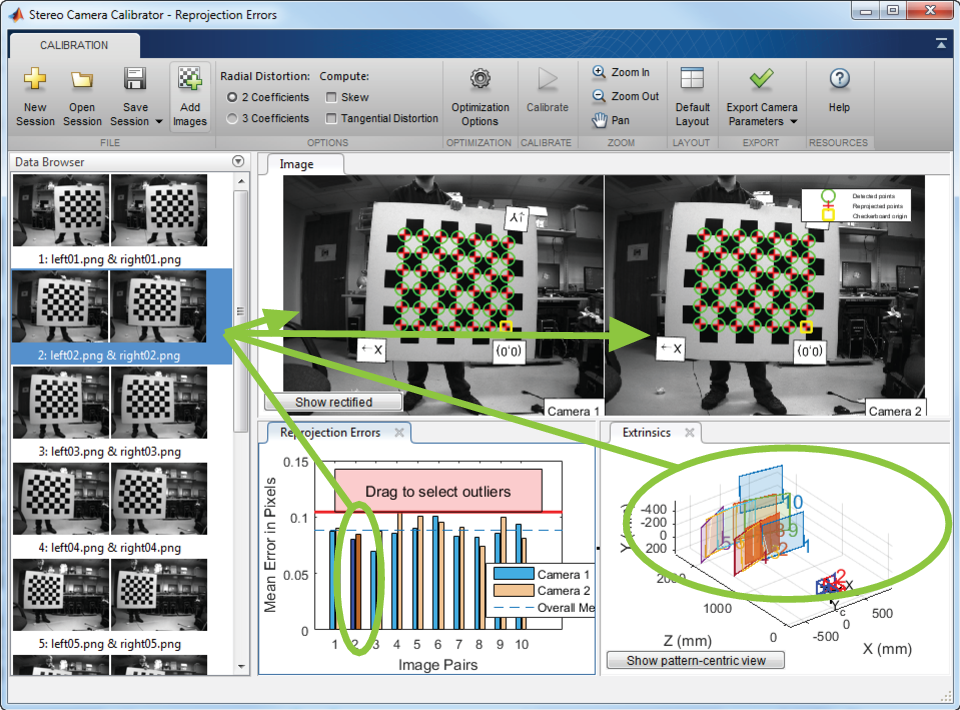
\includegraphics[width=1\textwidth]{./figures/stereocalibrator_selection.png}}
	\caption{Output of the Matlab calibration (Not me)}
	\label{fig:matlabcal}
\end{figure}

This gives a detailed view the error across the image set, as well as a 3D plot of the boards in 3D space. Dragging the bar on the re-projection graph allows you to single out bad images and remove them from the set to then run the calibration again. Repeat this until results are satisfactory.

\subsection{OpenCV Standard Model}

For a non stereo system calibartion looks like this 

\begin{lstlisting}[language=C++, frame=single, breaklines]
double rms = calibrateCamera(objectPoints, imagePoints, imageSize, K1, D1, rvec, tvec, flags, TermCriteria(3,20,1e-6));
\end{lstlisting}

This function takes in the vector objectPoints and imagePoints filled during corner detection, and outputs the values to the image Mats for the camera matrix and distortion matrix, K1 and D1 respectively. The flags field has a number of different options to fix values or increase the number of calculating coefficients, but they are usually not needed. The TermCriteria is what causes the calibration to stop and return a result. Its second parameter is the number of iterations it should try and fit the equation before stopping, and the third parameter is the error value it should return if it reaches a point below it. The first parameter simply says to stop when either condition is met, which is usually the option to take. Finally, the rms double being returned is the error being returned with a unit of pixels. As stated, the preferred amount it below 0.5.

For a stereo system there are just a few more parameters. 

\begin{lstlisting}[language=C++, frame=single, breaklines]
double rms = stereoCalibrate(objectPoints, leftImagePoints, rightImagePoints, K1, D1, K2, D2, imageSize, R, T, E, F, flags, TermCriteria(2,20,1e-6));
\end{lstlisting}

The only differences here are we have two images, two camera and distortion matrices being returned, and then a number of matrices used in the rectification calculations. Some additional flags the stereo function has are flags to fix parameters and read them in from a single calibration run done on the individual cameras. This has no alternative result, though, if you just ran the standard calibrate on each camera and passed their parameters in versus calculating them through the stereo calibration function. Rectification looks like this. 

\begin{lstlisting}[language=C++, frame=single, breaklines]
stereoRectify(K1, D1,K2,D2,imageSize,R,T,R1,R2,P1,P2,QQ,CALIB_ZERO_DISPARITY, 1, imageSize);
\end{lstlisting}

Here a new rectification transform and projection matrix are created so that images can be aligned. The Q matrix is also created and will be explained briefly later on. The \url{CALIB_ZERO_DISPARITY} flag aligns the principal points of each image, and the last two commands tell the image to not crop itself any and define the image resolution of the finished image respectively. 

To view the final image all that's left to do is create a new mapping matrix for which can map the old images to new undistorted ones. 

\begin{lstlisting}[language=C++, frame=single, breaklines]
initUndistortRectifyMap(K1, D1, R1, P1, imageSize, CV_32F, lmapx, lmapy);

remap(image, undistort_img, lmapx, lmapy, cv::INTER_LINEAR);
\end{lstlisting}
	
This pipeline results in a newly distorted image with error equivalent to that of the calibration. Because the coefficients are all the same across images taken with the same camera, once calibrated the matrices created can be saved and read in to run through initUndistortRectifyMap and remap on a different image set. Again this can all be found with more specific documentation at \url{http://docs.opencv.org/3.0-beta/modules/calib3d/doc/camera_calibration_and_3d_reconstruction.html}

\subsection{OpenCV Fisheye Model}

The fisheye model is really not very different.

\begin{lstlisting}[language=C++, frame=single, breaklines]
double rms = cv::fisheye::calibrate(objectPoints, leftImagePoints, imageSize, K1, D1, rvecs, tvecs, flag, cv::TermCriteria(3, 20, 1e-6));
\end{lstlisting}

\begin{lstlisting}[language=C++, frame=single, breaklines]
double rms = cv::fisheye::stereoCalibrate(objectPoints, leftImagePoints, rightImagePoints, K1, D1, K2, D2, imageSize, R, T, flag, cv::TermCriteria(3, 20, 1e-6));
\end{lstlisting}

\begin{lstlisting}[language=C++, frame=single, breaklines]
cv::fisheye::stereoRectify(K1, D1, K2, D2, imageSize, R, T, R1, R2, P1, P2, Q, cv::CALIB_ZERO_DISPARITY, imageSize, 0.0, 1.0);
\end{lstlisting}

The input is the same throughout. It is worth noting, though, that there are useful flags for better outcomes on the fisheye::stereoCalibrate. \url{CALIB_RECOMPUTE_EXTRINSIC} will recalculate the extrinsic result after each iteration of the calculation and \url{CALIB_CHECK_COND} will check if the condition number is valid. The condition number is a way of checking how right or wrong a coefficient matches an equation. This will check whether the result will most likely be horrible adjust. The same fisheye equivalent functions can be used to undistort any image once the coefficients are found. 

Some problems that can arise with the fisheye model are that a lot more safegaurds were put into place to check for bad output. Many crashes that may occur when running the fisheye model only occur because the results are so off. The regular calibration function just runs with these and returns large error while the fisheye model crashes. This is usually an indication that there are issues with your input images and you should do some debugging on the corner detection to see if something is wrong there. Again all this documentation can be found at \url{http://docs.opencv.org/3.0-beta/modules/calib3d/doc/camera_calibration_and_3d_reconstruction.html}

\subsection{Q Matrix}

For anyone doing image reconstruction after the fact, the reconstruction matrix, or Q matrix, genererated by the stereoRectify function is vital. In the case of working with Matlab, the Q matrix is not generated for you so you need to know how to put it together yourself. Not only that, but it is useful in understanding what the matrix means so that you can check if the output of your calibration actually makes logical sense. The Q matrix looks like this. 

\[ Q = 
\begin{bmatrix}
1 & 0 & 0 & -c_x \\ 0 & 1 & 0 & -c_y \\ 0 & 0 & 0 & f \\ 0 & 0 & \frac{-1}{T_x} & \frac{(c_x-c_x')}{T_x}
\end{bmatrix}
\]

Here c\textsubscript{x} and c\textsubscript{y} are the coordinates of the principal point of the left camera assuming stereo matching was left camera dominant. c'\textsubscript{x} is the x coorindate of the principal point in the right camera which should be the same in a perfect scenario or if \url{CV_CALIB_ZERO_DISPARITY} was flagged in stereoRectify. f is the focal length of the dominant camera, and T\textsubscript{x} is the baseline. The baseline can also be located as the first value in the translation vector between the coordinate systems of the camera. If this value is not close to what you measure with a ruler, there is obviously a problem. 

\section{References}

\begin{thebibliography}{9}
\bibitem{brown}
Brown, D. C.\textit{Close-range camera calibration}.
Photogrammetric Engineering, 37(8):855-866, 1971.

\bibitem{oldone}
Conrady, A. E.
\textit{Lens-systems, decentered}.
Monthly Notices of the Royal Astronomical Society, Vol. 79, p.384-390, 1919.

\bibitem{fisheye}
Kannala J, Brandt SS. 
\textit{A generic camera model and calibration method for conventional, wide-angle, and fish-eye lenses}. IEEE Trans Pattern Anal Mach Intell. 2006;28(8):1335-40.

\bibitem{matlab}
Matlab,\url{https://www.mathworks.com/help/vision/ug/camera-calibration.html}

\bibitem{opencv}
OpenCV,\url{http://docs.opencv.org/3.0-beta/modules/calib3d/doc/camera_calibration_and_3d_reconstruction.html}

\end{thebibliography}
	
\end{document}